\documentclass[12pt,a4paper]{ctexart}

\usepackage{amsmath,amssymb,bm,booktabs,caption,enumitem,fancyhdr,float,geometry,graphicx,hyperref,tcolorbox}

\geometry{left=25mm,right=25mm,top=25mm,bottom=25mm}
\graphicspath{{assets/figures/}}
\hypersetup{colorlinks=true,linkcolor=blue,citecolor=blue,urlcolor=blue}
\setlength{\parindent}{2em}
\setlength{\parskip}{0.35em}
\setlength{\headheight}{15pt}
\pagestyle{fancy}
\fancyhf{}
\lhead{Curved-Tube EP Flux}
\rhead{\thepage}

\newcommand{\p}{\partial}
\newcommand{\dd}{\,\mathrm d}
\newcommand{\D}{\mathrm D}
\newcommand{\mean}[1]{\left\langle #1\right\rangle_M}
\newcommand{\fluc}[1]{#1^{\dagger}}
\newcommand{\bt}{\boldsymbol t}
\newcommand{\be}{\boldsymbol e}
\newcommand{\br}{\boldsymbol r}
\newcommand{\bV}{\boldsymbol V}
\newcommand{\PP}{\boldsymbol{\mathsf P}_{\perp}}
\newcommand{\FF}{\mathsf F_{\mathrm{CT}}}
\newcommand{\RR}{\mathsf R}
\newcommand{\BB}{\boldsymbol B}
\newcommand{\PV}{\boldsymbol P}
\newcommand{\OO}{\Omega}
\newcommand{\GG}{\Gamma}
\newcommand{\LL}{\mathcal L}
\newcommand{\TT}{\mathcal T}

\title{\bfseries Curved-Tube EP Flux：\\弯曲材料涡管中的 E-P 通量推广}
\author{ZONCA-EP-FLUX}
\date{2026 年 8 月 31 日}

\begin{document}
\maketitle

\begin{tcolorbox}[colback=red!3,colframe=red!65!black,title={适用条件警告},fonttitle=\bfseries]
本文采用的是小曲率细涡管近似，核心几何量为
\[
  J=1-\kappa_\alpha x^\alpha .
\]
只有当 $\kappa r\ll1$ 且 $J>0$ 时，Bishop-frame 曲管坐标才可作为局地单射映射，
其 Jacobian/Christoffel 项才可进入近似闭合。当前全生命周期验证显示
$\epsilon_\kappa=\kappa r$ 的组合中位数约为 $10$ 到 $35$，且
metric valid fraction 的中位数为 $0$；因此本文的曲管项在这些样本中只能作为
几何风险审计，不能作为大曲率涡旋的闭合物理 forcing。大曲率版本应改用
\texttt{large\_curvature\_material\_volume\_ep\_flux.tex} 中的 Cartesian 材料体框架。
\end{tcolorbox}

本文档是 \texttt{E-P\_flux理论整理.tex} 的续篇，目标是把传统基于纬向平均和经圈平面
$(y,z)$ 的 E-P flux 思想，推广到三维中尺度涡的弯曲材料涡管。这里的 ``涡旋速度''
不再指相对于纬向平均的扰动，而是指相对于材料涡管截面平均的局地扰动。

\begin{tcolorbox}[colback=blue!3,colframe=blue!60!black,title={核心结论},fonttitle=\bfseries]
传统 E-P flux 的核心是把扰动动量通量和扰动热量通量合成为一个通量散度。
对弯曲三维涡旋，应把这个对象推广为沿材料涡管定义的张量通量
\[
  \FF^{ai}
  =
  -\rho_0 \mean{{u^\dagger}^{a}{u^\dagger}^{i}}
  +\rho_0\,\TT^{ia}\mean{{u^\dagger}^{a}\fluc{b}},
\]
其中 $a$ 是通量穿过的局地坐标方向，$i$ 是被强迫的动量或轴线速度分量，
$\TT^{ia}$ 是由 QG 热成风/PV 反演给出的浮力通量到平衡动量强迫的映射。
其协变散度
\[
  \nabla_a\FF^{ai}
  =
  J^{-1}\p_a(J\FF^{ai})
  +\Gamma^i{}_{ka}\FF^{ak}
\]
给出弯曲涡管内扰动对平均动量和 PV 矩心速度的净作用。涡旋轴线的倾斜和弯曲由
\[
  \D_t\bt=\PP\,\p_s\bV_c
\]
控制：只有轴线速度 $\bV_c$ 的轴向梯度中垂直于轴线的部分，才会真正改变涡旋轴方向。
\end{tcolorbox}

\section{为什么传统 E-P flux 不够}

传统 E-P flux 的平均算子是纬向平均，扰动定义为
\[
  \phi'=\phi-\overline{\phi}^{\,x}.
\]
这种定义隐含三个几何前提：第一，平均方向可以全局固定；第二，基本流和扰动的分离不随
涡旋轴线改变；第三，E-P flux 可以写成经圈平面中的二维向量
$\boldsymbol F=(F_y,F_z)$。

对一个三维中尺度涡，如果各层速度场的环流中心不在同一条竖直线上，甚至形成一条弯曲
空间曲线，这些前提都会失效。此时最重要的平均方向不再是纬向，而是随涡旋核心运动的
材料涡管；最重要的几何对象不再是固定 $(y,z)$ 平面，而是沿涡旋轴线移动的局地截面。

因此，推广的目标不是保留 $\overline{u'v'}$ 和 $\overline{v'T'}$ 的符号形式，而是保留
E-P 理论真正有价值的结构：
\begin{enumerate}[label=\arabic*.]
  \item 扰动动量通量和热量/浮力通量必须合成为同一个强迫对象；
  \item 这个强迫对象的散度，而不是通量本身，改变平均动量和平均 PV；
  \item 在平衡动力学中，PV 通量、浮力通量和动量通量不是独立诊断量。
\end{enumerate}

\section{材料弯曲涡管}

\subsection{轴线与 Bishop 标架}

令涡旋轴线为
\[
  \br_c=\br_c(s,t),
  \qquad
  \bt=\p_s\br_c,
  \qquad
  |\bt|=1,
\]
其中 $s$ 是沿轴线弧长。为避免 Frenet 标架在曲率很小时不稳定，采用 Bishop
或 rotation-minimizing 标架
\[
  \{\bt,\be_1,\be_2\},
  \qquad
  \p_s\bt=\kappa_\alpha\be_\alpha,
  \qquad
  \p_s\be_\alpha=-\kappa_\alpha\bt.
\]
局地坐标写为
\[
  \br(s,\xi,\eta,t)
  =
  \br_c(s,t)+\xi\be_1(s,t)+\eta\be_2(s,t).
\]
记 $x^1=\xi,\ x^2=\eta$，则一阶度量 Jacobian 为
\[
  J=1-\kappa_\alpha x^\alpha.
\]

\begin{figure}[H]
  \centering
  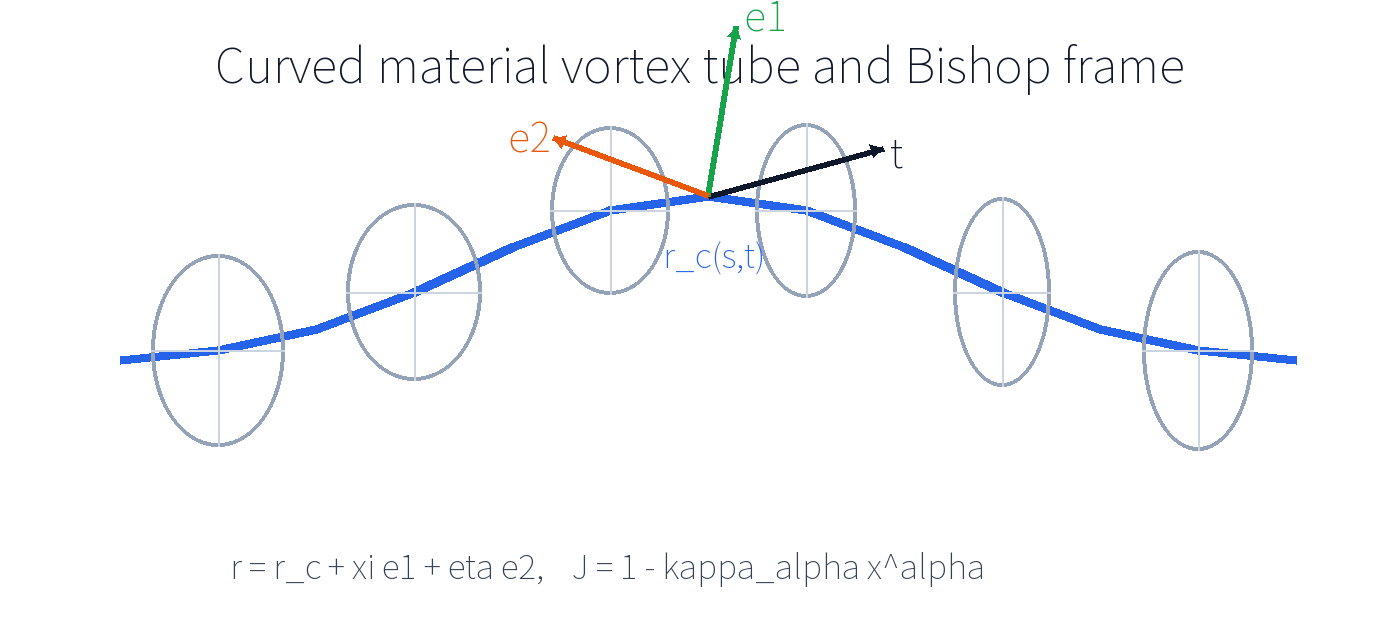
\includegraphics[width=0.92\linewidth]{ctep_tube_frame.png}
  \caption{弯曲材料涡管及 Bishop 标架。局地截面跟随轴线移动，曲率通过
  $J=1-\kappa_\alpha x^\alpha$ 进入面积和散度。}
\end{figure}

\subsection{材料 PV 等值边界}

令 $\OO(s,t)$ 是垂直于轴线的局地截面，$\GG(s,t)=\p\OO(s,t)$ 是任意闭合边界。
第一版模型把 $\GG$ 取为 coherent PV anomaly 的材料等值线或等值面，因此边界满足
\[
  \left(\boldsymbol u-\boldsymbol U_\GG\right)\cdot\boldsymbol n_\GG=0,
\]
即没有普通的边界穿透通量。边界可以非圆、偏心或拉伸；这些形变不被先验抹平，
而是保留在截面积分、边界积分和 Jacobian 中。

\subsection{PV 矩心轴线}

令 $q_c$ 表示用于定义 coherent 本体的有符号 PV anomaly。截面 PV 质量为
\[
  M_q(s,t)=\int_{\OO(s,t)}q_cJ\dd A.
\]
涡旋轴点定义为 PV 矩心
\[
  \br_c(s,t)
  =
  \frac{\int_{\OO(s,t)}\br\,q_cJ\dd A}{\int_{\OO(s,t)}q_cJ\dd A}.
\]
等价地，在局地截面坐标中要求
\[
  \int_{\OO(s,t)}\boldsymbol x_\perp q_cJ\dd A=0,
  \qquad
  \boldsymbol x_\perp=\xi\be_1+\eta\be_2.
\]

\begin{figure}[H]
  \centering
  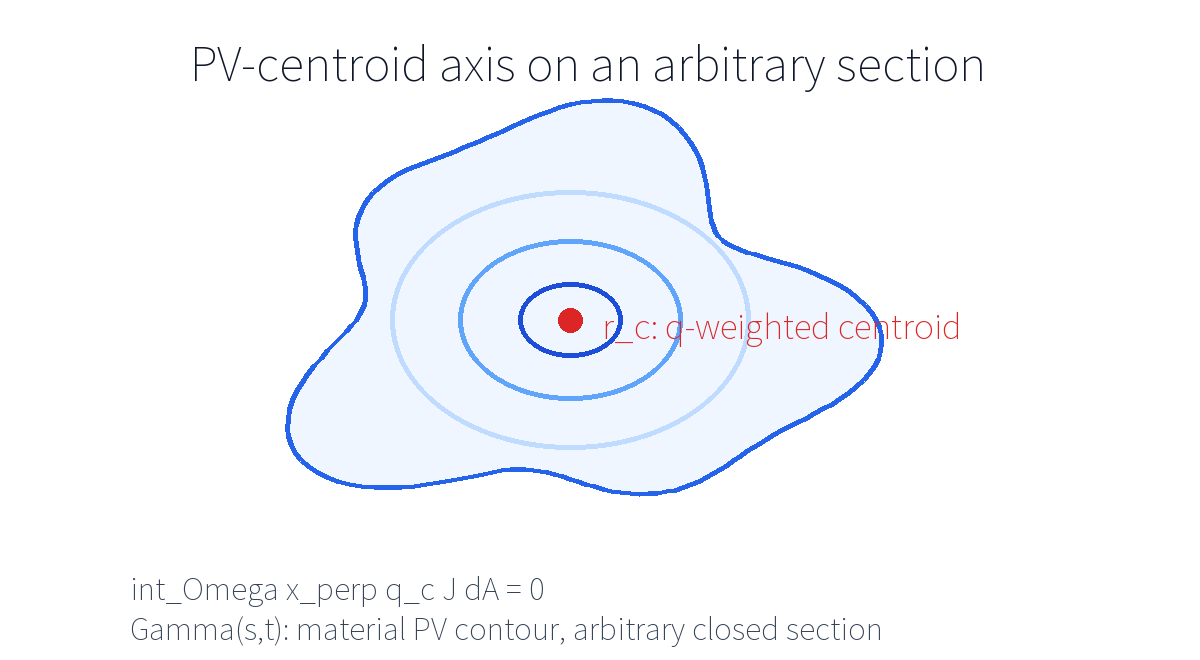
\includegraphics[width=0.80\linewidth]{ctep_pv_centroid.png}
  \caption{任意闭合截面上的 PV 矩心。涡旋轴线不是几何圆心连线，而是 coherent PV anomaly
  的加权矩心连线。}
\end{figure}

\section{材料平均与扰动定义}

对任意物理量 $\phi$，定义材料管截面平均
\[
  A(s,t)=\int_{\OO(s,t)}J\dd A,
  \qquad
  \mean{\phi}
  =
  \frac{1}{A(s,t)}\int_{\OO(s,t)}\phi J\dd A.
\]
扰动定义为
\[
  \fluc{\phi}=\phi-\mean{\phi},
  \qquad
  \mean{\fluc{\phi}}=0.
\]
这个定义替代传统纬向平均。它的物理意义是：涡旋的 ``平均状态'' 是随 coherent 涡管
运动的截面平均，扰动是截面内的非轴对称结构、内部波动、局地剪切和高阶形变。

对速度分量，采用 Bishop 标架展开
\[
  \boldsymbol u=u^s\bt+u^1\be_1+u^2\be_2.
\]
其中 $u^s$ 是沿轴流动，$u^1,u^2$ 是截面内运动。后续所有二阶通量都使用
${u^\dagger}^i$，而不是传统 $u'$。

\section{QG/Boussinesq 动力近似}

第一版保留 ocean QG/Boussinesq 层级。以浮力
\[
  b=-g\rho'/\rho_0
\]
为热变量。直角坐标下的 QG PV 可写为
\[
  q
  =
  \nabla_h^2\psi
  +
  \p_z
  \left(
    \frac{f_0^2}{N^2}\p_z\psi
  \right)
  +\beta y.
\]
在弯曲涡管坐标中，将其写成形式不变但含度量修正的反演关系
\[
  q=\LL_g\psi+\beta y,
\]
其中
\[
  \LL_g\psi
  =
  J^{-1}\p_a\left(JG^{ab}\p_b\psi\right)
  +
  \p_z\left(\frac{f_0^2}{N^2}\p_z\psi\right)
  +
  \mathcal O(\kappa_\alpha x^\alpha,\p_s\kappa_\alpha).
\]
若轴线变直、$J\to1$、曲率项消失，则 $\LL_g$ 退化为通常的 QG PV 反演算子。

\section{扰动通量张量}

传统 E-P flux 把 $\overline{u'v'}$ 与 $\overline{v'T'}$ 合成二维向量。在材料弯曲涡管中，
方向不再只有 $y,z$，被强迫的动量分量也不再只是一维纬向动量。因此自然对象是二阶通量张量。

定义材料 Reynolds stress
\[
  \RR^{ai}
  =
  \mean{{u^\dagger}^{a}{u^\dagger}^{i}},
  \qquad
  a,i\in\{s,1,2\}.
\]
定义浮力通量
\[
  B^a
  =
  \mean{{u^\dagger}^{a}\fluc{b}},
\]
以及 PV 通量
\[
  P^a
  =
  \mean{{u^\dagger}^{a}\fluc{q}}.
\]
其中 $a$ 是 ``穿过哪个局地坐标方向输送''，$i$ 是 ``哪个动量分量被输送''。

PV 通量是轴线动力最直接的对象；Reynolds stress 与浮力通量则是与传统 E-P 理论衔接的对象。
QG 平衡把三者联系起来：浮力通量通过热成风关系改变平衡剪切，PV 通量通过反演改变涡旋
诱导速度，动量通量通过应力散度改变平均速度。

\section{Curved-Tube EP flux 张量}

定义 Curved-Tube EP flux 张量为
\[
  \boxed{
  \FF^{ai}
  =
  -\rho_0\RR^{ai}
  +
  \rho_0\,\TT^{ia}B^a
  }
\]
这里 $\TT^{ia}$ 是平衡映射算子：它把浮力通量 $B^a$ 转化为对第 $i$ 个动量分量的平衡强迫。
它是传统 E-P flux 中
\[
  F_z\propto \frac{f_0}{N^2}\overline{v'T'}
\]
在弯曲坐标中的推广。也就是说，$\FF^{ai}$ 不是简单的 Reynolds stress；它是
``动量通量 + 由浮力通量经平衡关系折算出的动量强迫''。

其协变散度为
\[
  \nabla_a\FF^{ai}
  =
  J^{-1}\p_a(J\FF^{ai})
  +
  \Gamma^i{}_{ka}\FF^{ak}.
\]
第一项是带 Jacobian 的通量散度，第二项是曲线坐标中的几何联络项。当轴线有曲率时，
即使 $\FF^{ai}$ 在局地坐标中看似均匀，几何项也可能产生有效强迫。

\begin{figure}[H]
  \centering
  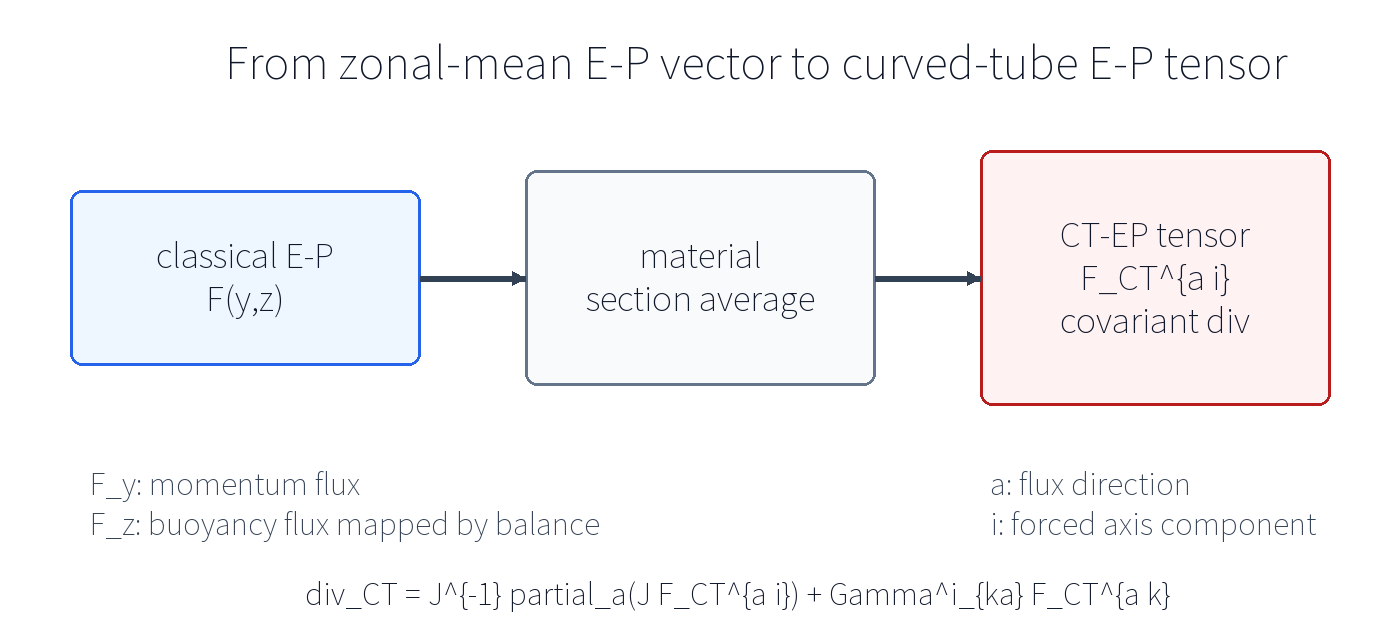
\includegraphics[width=0.92\linewidth]{ctep_tensor_upgrade.png}
  \caption{从传统 E-P 向量到 Curved-Tube EP 张量。推广的重点是替换平均算子和散度算子，
  而不是简单替换符号。}
\end{figure}

材料管平均动量方程的诊断形式可写为
\[
  \frac{\D_M\mean{u^i}}{\D t}
  +
  \mathcal C^i_{\mathrm{geom}}
  =
  \rho_0^{-1}\nabla_a\FF^{ai}
  +
  \mathcal S^i_{\mathrm{ageo}}
  +
  \mathcal S^i_{\mathrm{mix}}.
\]
$\mathcal C^i_{\mathrm{geom}}$ 包含曲率、度量和随轴标架旋转导致的表观项；
$\mathcal S^i_{\mathrm{ageo}}$ 表示年龄转或非 QG 残差；
$\mathcal S^i_{\mathrm{mix}}$ 表示混合、摩擦和非保守过程。第一版理论中，真正的 E-P 型
诊断量是 $\rho_0^{-1}\nabla_a\FF^{ai}$。

\section{轴线演化方程}

从 PV 矩心定义
\[
  \int_{\OO}\boldsymbol x_\perp q_cJ\dd A=0
\]
出发，对时间求导。若边界为材料 PV 等值面，则普通边界穿透通量为零，轴线速度可以写成
\[
  \bV_c
  =
  \frac{1}{M_q}
  \int_{\OO}\boldsymbol u\,q_cJ\dd A
  +
  \frac{1}{M_q}
  \int_{\OO}\boldsymbol x_\perp S_qJ\dd A
  +
  \boldsymbol V_{\mathrm{geom}},
\]
其中 $S_q$ 是非保守 PV 源，$\boldsymbol V_{\mathrm{geom}}$ 是曲率和截面形变带来的度量修正。
将速度和 PV 分解为材料平均与扰动，可得
\[
  V_c^i
  =
  \mean{u^i}
  +
  \frac{A}{M_q}\mean{{u^\dagger}^i\fluc{q_c}}
  +
  V_{\mathrm{src}}^i
  +
  V_{\mathrm{geom}}^i.
\]
这说明涡旋轴线漂移不仅由截面平均速度给出，还由 PV 通量协方差
$\mean{{u^\dagger}^i\fluc{q_c}}$ 给出。通过 QG PV 反演，这个 PV 通量又可由
Curved-Tube EP flux 散度诊断。

令轴线切向量 $\bt=\p_s\br_c$。对 $\bt$ 作材料导数：
\[
  \D_t\bt
  =
  \p_s\bV_c
  -
  \left(\bt\cdot\p_s\bV_c\right)\bt
  =
  \PP\,\p_s\bV_c,
\]
其中
\[
  \PP=\boldsymbol I-\bt\bt
\]
是投影到法平面的算子。这就是弯曲三维涡旋最重要的结果：沿轴速度剪切的切向分量只改变
参数化速度，法向分量才改变轴线方向。

把上式与 CT-EP 诊断联系起来，可写成
\[
  \D_t\bt
  =
  \PP\,\p_s
  \left[
    \mean{\boldsymbol u}
    +
    \frac{A}{M_q}\boldsymbol P_q
    +
    \rho_0^{-1}\mathcal K
    \left(\nabla_a\FF^{a\cdot}\right)
    +
    \boldsymbol V_{\mathrm{src}}
    +
    \boldsymbol V_{\mathrm{geom}}
  \right],
\]
其中
\[
  \boldsymbol P_q
  =
  \mean{\fluc{\boldsymbol u}\fluc{q_c}},
\]
$\mathcal K$ 表示由 QG PV 反演和热成风平衡给出的速度响应算子。这条式子是本理论的主方程：
通量散度并不只是加速某个固定方向的平均流，而是通过改变 PV 矩心速度的轴向梯度，驱动
涡旋轴线倾斜、弯曲和漂移。

\begin{figure}[H]
  \centering
  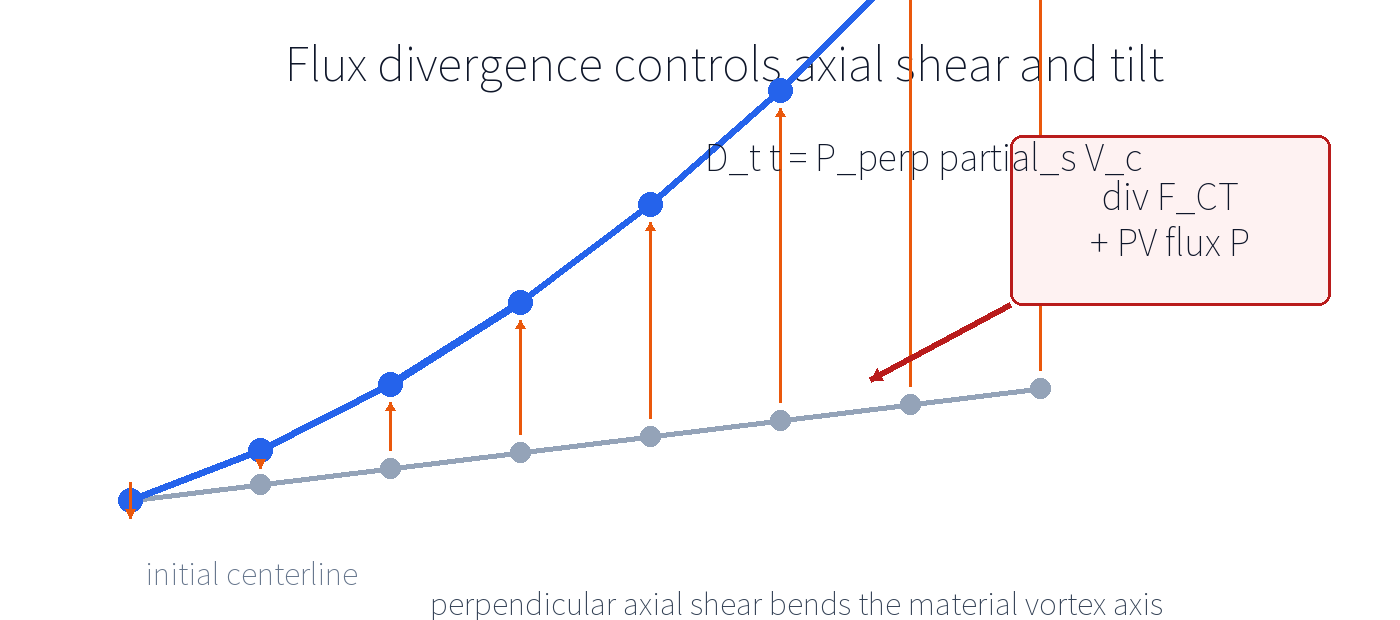
\includegraphics[width=0.90\linewidth]{ctep_axis_evolution.png}
  \caption{CT-EP 通量散度和 PV 通量改变 $\p_s\bV_c$，其法向投影驱动轴线倾斜与弯曲。}
\end{figure}

\section{与传统 E-P flux 的对应极限}

若轴线变直、$\kappa_\alpha=0$、$J=1$，截面为圆或统计轴对称，平均算子退化为固定方向
平均，并且只关心一个被强迫的平均动量分量，则
\[
  \nabla_a\FF^{ai}
  \longrightarrow
  \p_yF_y+\p_zF_z,
\]
并恢复传统 TEM/E-P flux 的结构：
\[
  \frac{\p\overline{u}}{\p t}-f_0v^*
  =
  \rho_0^{-1}\nabla\cdot\boldsymbol F+\overline X.
\]
因此，Curved-Tube EP flux 不是另起炉灶，而是把传统 E-P 理论中
``通量组合 - 散度强迫 - PV 反演反馈'' 的核心结构搬到弯曲材料涡管上。

\section{第一版诊断步骤}

后续若进入数值诊断，可按以下顺序实现：
\begin{enumerate}[label=\arabic*.]
  \item 用 $q_c$ 或 $\psi_c$ 识别 coherent PV 核，并确定材料边界 $\GG(s,t)$；
  \item 在每个截面计算 PV 矩心 $\br_c(s,t)$，构造 Bishop 标架；
  \item 用材料截面平均得到 $\mean{\phi}$ 和 $\fluc{\phi}$；
  \item 计算 $\RR^{ai}$、$B^a$、$P^a$；
  \item 通过 QG 平衡映射构造 $\FF^{ai}$；
  \item 计算协变散度 $\nabla_a\FF^{ai}$；
  \item 诊断 $\bV_c$ 与 $\D_t\bt=\PP\p_s\bV_c$，判断倾斜、弯曲和 coherent 失稳位置。
\end{enumerate}

\section{开放项}

第一版理论保留三个开放项：
\begin{enumerate}[label=\arabic*.]
  \item $\TT^{ia}$ 的具体离散形式应由所用 QG PV 反演和网格坐标决定；
  \item $\boldsymbol V_{\mathrm{geom}}$ 对强曲率涡管可能不小，需要在数值实现时单独验证；
  \item 非保守 PV 源 $S_q$ 会直接移动 PV 矩心，不能简单并入 E-P 通量散度。
\end{enumerate}

\section{一句话总结}

Curved-Tube EP Flux 的精髓是：对弯曲三维中尺度涡，不能再用纬向平均下的二维 E-P flux
描述波-平均流相互作用；应在 coherent PV 材料涡管内定义截面平均和扰动，把扰动动量通量
与浮力通量合成为局地张量 $\FF^{ai}$，再用其协变散度和 PV 通量解释涡旋轴线速度
$\bV_c$ 的轴向变化。最终控制 coherent tilt 和弯曲的不是某一层水平速度或垂直速度本身，
而是
\[
  \PP\,\p_s\bV_c.
\]

\end{document}
